%\section{Lensed waveguide}
%lensed_waveguide
In this section we will discuss another important waveguide structure for efficient coupling. In many articles it has been well discussed about the coupling between laser source and lensed fiber\cite{microlensese_to_fiber_coupling} and \cite{integrated_coupling _between_LD_SMF}.  Edward in \cite{microlensese_to_fiber_coupling} provided a microlens design for coupling lasers to fibers. The coupling efficiency in his work reaches maximum about $56\%$. SHIRAISHI has also presented in \cite{integrated_coupling _between_LD_SMF} some lensed fiber designs and has gained a minimum coupling loss less than $2$dB with those microlens designs. It brings us a idea, by means of mounting a microlens on the waveguide interface we could gain higher performance by the use of a microlens at the interface of the waveguide. For the fabrication it may be not easy to mount a microlens on a stript rib waveguide. But in \cite{lens_end_manufacture} the process sequence for fabricating the lens on the fiber end brings us the possibility to create a lens on a buried waveguide. In this section the coupling efficiency between TLF and the lensed buried waveguide (or lensed waveguide) Fig. \ref{fig:lensed_waveguide} will be discussed.
In the first subsection we will calculate the coupling efficiency between TLF and regular buried waveguide as the reference for further discussing. Then we can continue to talk about the lensed waveguide and the effect of varying the lens geometric ($h'$ and $R$) parameters of the lensed waveguide. 
\begin{figure}[!ht]
\centering
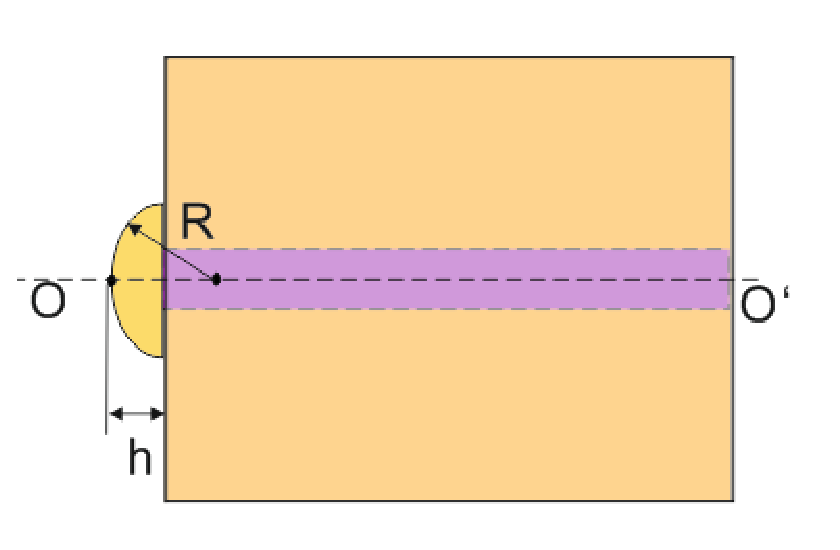
\includegraphics[width=0.7\textwidth]{bilder/lensed_waveguide}
\caption{Schema of a lensed buried waveguide.}
\label{fig:lensed_waveguide}
\end{figure}
